
%(BEGIN_QUESTION)
% Copyright 2015, Tony R. Kuphaldt, released under the Creative Commons Attribution License (v 1.0)
% This means you may do almost anything with this work of mine, so long as you give me proper credit

Examine this schematic diagram of a protective relay system, from page 138 of {\it Protective Relays} by Victor H. Todd (published in 1922):

$$\includegraphics[width=15.5cm]{i02874x01.eps}$$

First, identify the type of system protection provided by this relay circuit.  Next, explain the function of the auxiliary switch shown in the diagram.

\vskip 10pt

\underbar{file i02874}
%(END_QUESTION)





%(BEGIN_ANSWER)

This is some form of overcurrent protection, either 50, 51, or both.  The oil circuit breaker gets tripped if either of the two protective relays senses an overcurrent condition and closes its trip contact.

\vskip 10pt

The auxiliary switch interrupts (breaks) the trip function when actuated.  This is actually the 52a contact on the oil circuit breaker, but the schematic diagram isn't perfectly clear on this point so it's okay if students don't recognize its true function (auxiliary to the breaker) and see it as a manually actuated switch (used to facilitate maintenance work on the relays with the breaker closed?).

%(END_ANSWER)





%(BEGIN_NOTES)

{\bf This question is intended for exams only and not worksheets!}.

%(END_NOTES)


